\documentclass[10pt,a4paper]{article}
\usepackage[utf8]{inputenc}
\usepackage[T1]{fontenc}
\usepackage{amsmath}
\usepackage{amsfonts}
\usepackage{amssymb}
\usepackage{graphicx}
\usepackage{indentfirst}
\usepackage{etoolbox}
\usepackage{placeins}
\usepackage{subcaption}

\usepackage[style=ieee, backend=bibtex ,sorting=none]{biblatex}
\addbibresource{refs.bib}
%opening
\author{Piotr Kumala}
\title{Zastosowanie rekurencyjnych sieci neuronowych do predykcji szeregów czasowych}
\date{}
\graphicspath{ {./img/} }
\renewcommand*\contentsname{Spis treści}
\renewcommand*\figurename{Rysunek}

\begin{document}
\begin{titlepage}
	\begin{center}
		
\includegraphics[width=0.4\textwidth]{img/university.jpg}
		\vspace*{1cm}
		
		{\Huge
			\textbf{Praca magisterska} \\
			
		}
		\vspace{0.5cm}
		{\Large
			Zastosowanie rekurencyjnych sieci neuronowych do predykcji szeregów czasowych
			
			\vspace{1cm}
			
			\textbf{Piotr Kumala} \\
		}
		\vspace{0.5cm}
		kierunek studiów: \textbf{Informatyka Stosowana} \\
		
		\vspace{1cm}
		
		{\Large Opiekun: \textbf{dr hab. inż. Piotr A. Kowalski}}
		\vfill
		
		\
		\vspace{0.8cm}
		
		
		Wydział Fizyki i Informatyki Stosowanej\\
		Akademia Górniczo-Hutnicza im. Stanisława Staszica\\
		Kraków, lipiec 2021r.
		
	\end{center}
\end{titlepage}
\pagenumbering{gobble}
\newpage
\begin{center}
	\textbf{Oświadczenie studenta}
\end{center}

Uprzedzony o odpowiedzialności karnej na podstawie art. 115 ust. 1 i 2 ustawy z dnia
4 lutego 1994 r. o prawie autorskim i prawach pokrewnych (t.j. Dz. U. z 2018 r. poz. 1191 z
późn. zm.): „Kto przywłaszcza sobie autorstwo albo wprowadza w błąd, co do autorstwa całości
lub części cudzego utworu albo artystycznego wykonania, podlega grzywnie, karze
ograniczenia wolności albo pozbawienia wolności do lat 3. Tej samej karze podlega, kto
rozpowszechnia bez podania nazwiska lub pseudonimu twórcy cudzy utwór w wersji
oryginalnej albo w postaci opracowania, artystyczne wykonanie albo publicznie zniekształca
taki utwór, artystyczne wykonanie, fonogram, wideogram lub nadanie.”, a także uprzedzony o
odpowiedzialności dyscyplinarnej na podstawie art. 307 ust. 1 ustawy z dnia 20 lipca 2018r.
Prawo o szkolnictwie wyższym i nauce (Dz. U. z 2018 r. poz. 1668 z późn. zm.) „Student
podlega odpowiedzialności dyscyplinarnej za naruszenie przepisów obowiązujących w uczelni
oraz za czyn uchybiający godności studenta.”, oświadczam, że niniejszą pracę dyplomową
wykonałem osobiście i samodzielnie i nie korzystałem ze źródeł innych niż wymienione w
pracy. 

Jednocześnie Uczelnia informuję, że zgodnie z art. 15a ww. ustawy o prawie autorskim
i prawach pokrewnych Uczelni przysługuje pierwszeństwo w opublikowaniu pracy
dyplomowej studenta. Jeżeli Uczelnia nie opublikowała pracy dyplomowej w terminie 6
miesięcy od dnia jej obrony, autor może ją opublikować chyba, że praca jest częścią utworu
zbiorowego. Ponadto Uczelnia, jako podmiot, o którym mowa w art. 7 ust. 1 pkt 1 ustawy z
dnia 20 lipca 2018 r. — Prawo o szkolnictwie wyższym i nauce (Dz. U. z 2018 r. poz. 1668 z
późn. zm.), może korzystać bez wynagrodzenia i bez konieczności uzyskania zgody autora z
utworu stworzonego przez studenta w wyniku wykonywania obowiązków związanych z
odbywaniem studiów, udostępnić utwór ministrowi właściwemu do spraw szkolnictwa
wyższego i nauki oraz korzystać z utworów znajdujących się w prowadzonych przez niego
bazach danych, w celu sprawdzania z wykorzystaniem systemu antyplagiatowego. Minister
właściwy do spraw szkolnictwa wyższego i nauki może korzystać z prac dyplomowych
znajdujących się w prowadzonych przez niego bazach danych w zakresie niezbędnym do
zapewnienia prawidłowego utrzymania i rozwoju tych baz oraz współpracujących z nimi
systemów informatycznych.

\vfill
\
\begin{flushright}
	............................................................... \\
	(czytelny podpis)
\end{flushright}

\newpage
\pagenumbering{arabic}
\tableofcontents
\newpage

\section{Wprowadzenie i cel pracy}

\subsection{Wprowadzenie}
Sieci neuronowe są coraz powszechniej używane do rozwiązywania wielu problemów życia codziennego. Nawet w wydawałoby się prostych urządzeniach jak telefony komórkowe zawierane są układy elektroniczne specjalizujące się w obliczeniach korzystających z sieci neuronowych \cite{appleNeuralEngine}. Taki rozwój technologiczny może zostać zastosowany do próby zrozumienia i szukania rozwiązań problemów życia codziennego. Jednym z szeroko występujących w świadomości społecznej problemów jest poziom zanieczyszczenia środowiska naturalnego i zmiany klimatu. Co roku na początku zimy media raportują o wysokim poziome zanieczyszczeń powietrza w polskich miastach. Podejmowane są również działania mające na celu ograniczenie poziomu tychże zanieczyszczeń przez samorządy i instytucje centralne. Posiadanie wiarygodnych estymacji skali problemu i jego zmiany w czasie może mieć wymierne skutki w usprawnianiu reakcji na wysokie poziomy zanieczyszczeń. W tej pracy podjęta zostanie próba stworzenia wiarygodnego modelu predykcyjnego poziomu zanieczyszczeń korzystającego z rekurencyjnych sieci neuronowych.

\subsection{Cel pracy}
Rekurencyjne sieci neuronowe są szeroko wykorzystywane i rozwijane przez największe firmy technologiczne. Są one stosowane między innymi do rozpoznawania pisma odręcznego i tekstu dyktowanego (Google Android LSTM). Mając na uwadze ilość wysiłku wkładanego w ulepszanie tychże sieci nasuwa się pytanie jakie rezultaty będą one osiągać w innych zastosowaniach. W ramach tej pracy zbadana zostanie jakość predykcji szeregów czasowych płynących z modeli opartych na rekurencyjnych sieciach neuronowych. Zostaną one zestawione z klasycznymi metodami predykcyjnymi w celu stwierdzenia zasadności stosowania sieci neuronowych. Specjalna uwaga zostanie również poświęcona różnicom w jakości uzyskiwanych rozwiązań różnych architektur sieci oraz skalowalności modeli opartych na rekurencyjnych sieciach neuronowych. 

\section{Wstęp teoretyczny}
\subsection{Szereg czasowy}
W ramach pracy podejmowane będą próby predykcji szeregu czasowego. Przed rozpoczęciem dalszych dywagacji należy zdefiniować samo pojęcie aby uniknąć nieścisłości. Podążając za Głównym Urzędem Statystycznym szeregiem czasowym nazywamy ciąg obserwacji ilustrujący kształt zjawiska w kolejnych okresach czasu. Obserwacją można określić zbiór cech opisujących zjawisko w danym punkcie czasu. Rozumiejąc w taki sposób pojęcie szeregu czasowego można w prosty sposób określić cel systemu predykcyjnego. System ten powinien być w stanie przewidzieć wartość pewnej cechy w kolejnym punkcie czasu na podstawie poprzednich obserwacji. Można również określić, że predykcja będzie tym lepsza im bardziej zgodna z posiadanymi obserwacjami. 

\subsection{Regresja liniowa}
Jedną z najbardziej klasycznych metod predykcyjnych jest regresja liniowa. Jej podstawy zostały położone w pracach Legrende'a i Gauss'a na początku XIX wieku \cite{seal1967studies}. Polega ona na dopasowywaniu funkcji liniowej do danych w taki sposób, aby jak najlepiej opisywała ona kształt i właściwości danych. Najprostszym mechanizmem służącym do zapewnienia optymalnych wyników jest metoda najmniejszych kwadratów opisana po raz pierwszy przez Legrende'a w 1805 roku\cite{legendre1806nouvelles}. Polega ona na takim dopasowywaniu parametrów funkcji aby zminimalizować sumaryczny kwadrat odległości obserwacji od prostej opisanej funkcją. 
\begin{figure}[!ht]
	\centering
	\makebox[0pt]{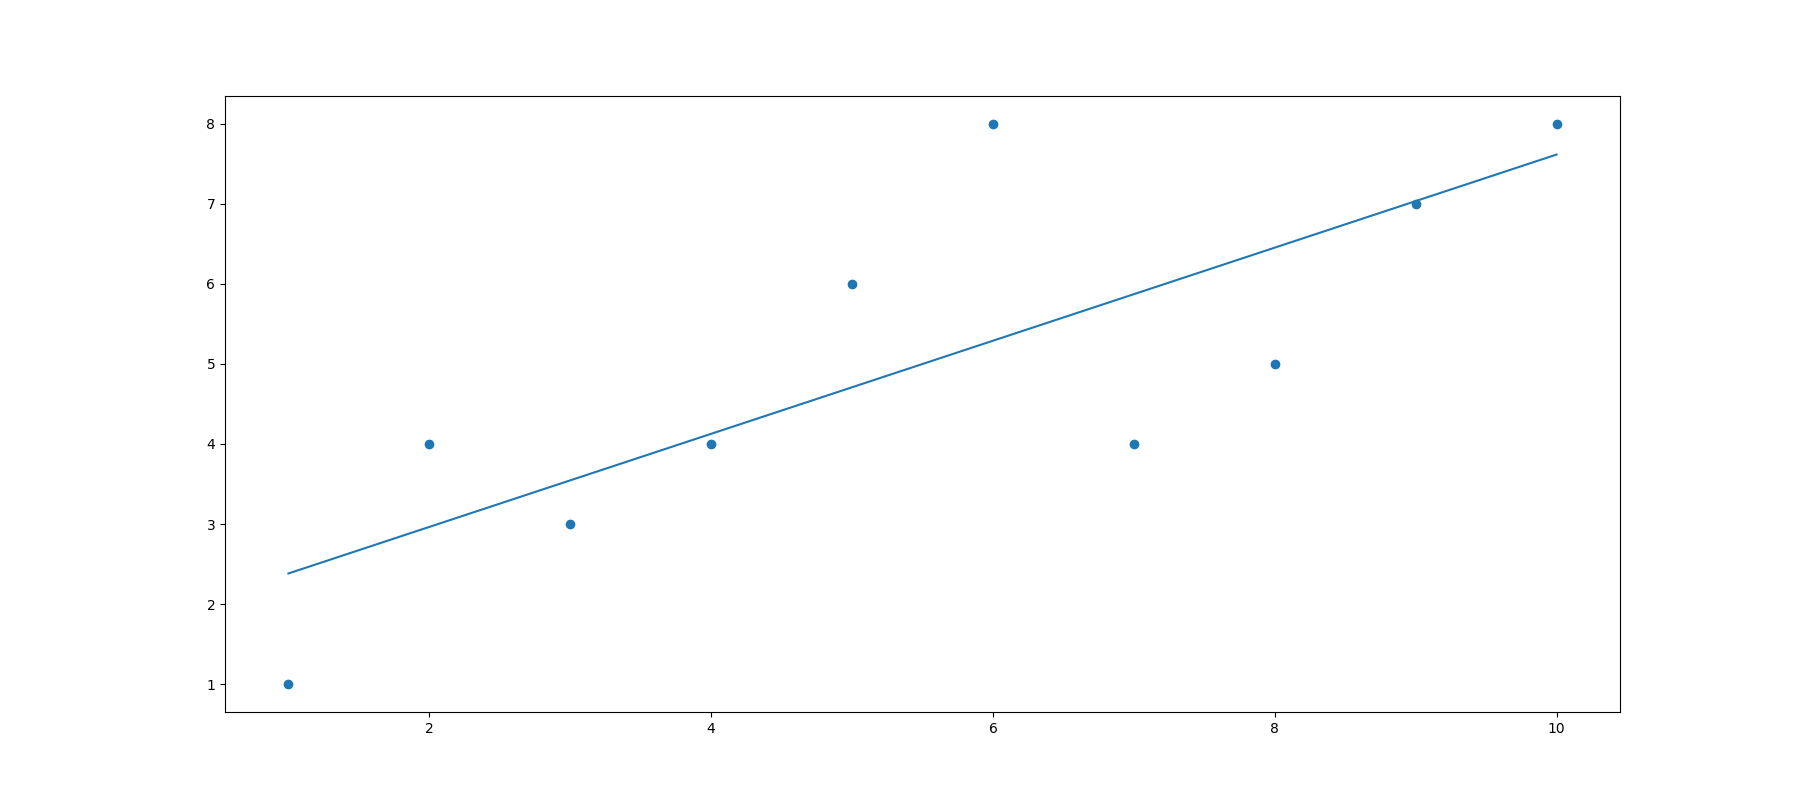
\includegraphics[scale=0.2]{example_linear_regression.png}}
	\caption{Przykład wyniku regresji liniowej}
\end{figure}
\FloatBarrier
Metoda ta jest szeroko wykorzystywana, ale nie jest pozbawiona wad. Bardzo mocno reaguje ona na elementy nietypowe co może prowadzić do nieprawidłowego kształtu funkcji. F. Anscombe  w 1973 roku zaprezentował cztery zbiory danych, które korzystając z metody najmniejszych kwadratów zwracają takie same proste pomimo tego, że kształty tychże zbiorów danych są bardzo od siebie różne \cite{anscombe1973graphs}.
\begin{figure}[!ht]
	\centering
	\makebox[0pt]{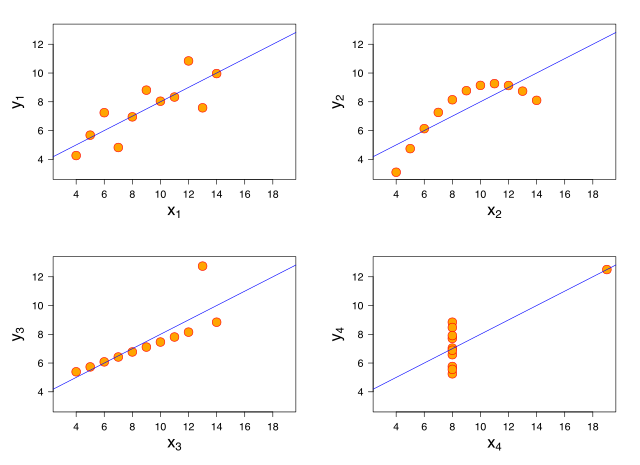
\includegraphics[scale=0.6]{anscombe.png}}
	\caption{Zbiory opisane przez Anscombe'ego i dopasowane do nich proste}
\end{figure}
\FloatBarrier 
\subsection{Drzewa decyzyjne}
Jedną z najszerzej używanych metod uczenia maszynowego są drzewa decyzyjne. Są one szeroko wykorzystywane ze względu na swoje nieskomplikowanie i intuicyjność w zrozumieniu wyników \cite{wu2008top}. Drzewem decyzyjnym nazywamy model predykcyjny, $h: X \rightarrow Y$, który przewiduje wartość $Y$ dla $x$ poprzez trawers drzewa od korzenia do liścia. Na każdym węźle drzewa kierunek przejścia jest wybierany poprzez rozdzielenie przestrzeni wejściowej. Najczęściej jest ono dokonywane na podstawie cech obserwacji $x$ \cite{books/daglib/0033642}. Wynikiem procesu uczenia jest drzewo pozwalające prześledzić ścieżkę jaką podąża każda obserwacja $x$ w celu przypisania jej odpowiedniej wartości. Przykładowe, bardzo uproszczone drzewo decyzyjne jest przedstawione na rysunku numer 3.
\begin{figure}[!ht]
	\centering
	\makebox[0pt]{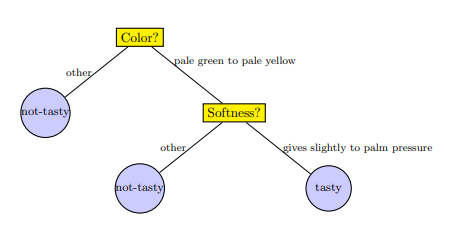
\includegraphics[scale=0.8]{example_decission_tree.png}}
	\caption{Przykładowe drzewo decyzyjne}
\end{figure}
\FloatBarrier

Na podstawie tego przykładu można łatwo zaobserwować główną zaletę drzew decyzyjnych, mianowicie łatwość interpretacji uzyskanego drzewa. Podejmowanie decyzji poprzez odpowiadanie na pytania, które stale zawężają możliwe rozwiązania jest intuicyjnie zrozumiałe. Powodem tej łatwości zrozumienia może być bliskość procesu wyboru przez drzewo do ludzkiego procesu podejmowania decyzji. Niektórzy ludzie twierdzą, że drzewo decyzyjne powiela ludzkie schematy myślowe \cite{James2013}. 

Drzewa decyzyjne mogą być wykorzystywane w problemach regresyjnych to znaczy dla ciągłej dziedziny rozwiązań $Y$. Należy jednak pamiętać, że w takim przypadku  należy uważać na możliwość zbytniego dopasowywania drzewa do danych trenujących. Problem ten objawia się stworzeniem zbyt szczegółowego drzewa, które nie generalizuje odpowiednio danych nieobecnych w zbiorze treningowym.

\subsection{Rekurencyjne sieci neuronowe}
Rekurencyjne sieci neuronowe to sieci neuronowe posiadające pętlę sprzężenia zwrotnego w swojej warstwie rekurencyjnej. Taka struktura pozwala im ,,zapamiętywać'' informacje przez pewien okres czasu i wykorzystywać w dalszych predykcjach \cite{reviewOfANN2018}. Taka umiejętność pozwala przewidywać, że rekurencyjna sieć neuronowa powinna dobrze zachowywać się w predykcji szeregu czasowego dzięki ,,zapamiętywaniu'' wartości w poprzednich krokach czasowych. 

Podwaliny rekurencyjnych sieci neuronowych zostały stworzone w 1986 roku przez D. Rumelhart'a. Opisywał on sposób uczenia sieci neuronowych poprzez propagację wsteczną błędu \cite{rumelhart1986learning}. Zauważył on, że korzystając z tej metody uczenia można wypracować sieć, która rekurencyjnie wyznaczy wartości wag neuronów w swojej warstwie ukrytej. Potrzeba opracowania nowego sposobu uczenia wynikała z istnienia zadań niedających się rozwiązać poprzez proste połączenie jednostek wejściowych z wyjściowymi.

Powszechnym sposobem myślenia o strukturze sieci neuronowych jest seria warstw składających się na sieć. Każda warstwa składająca się z pewnej liczby neuronów komunikuje się z następującą warstwą aż do osiągnięcia warstwy wyjściowej zwracającej wynik sieci. 
\begin{figure}[!ht]
	\centering
	\makebox[0pt]{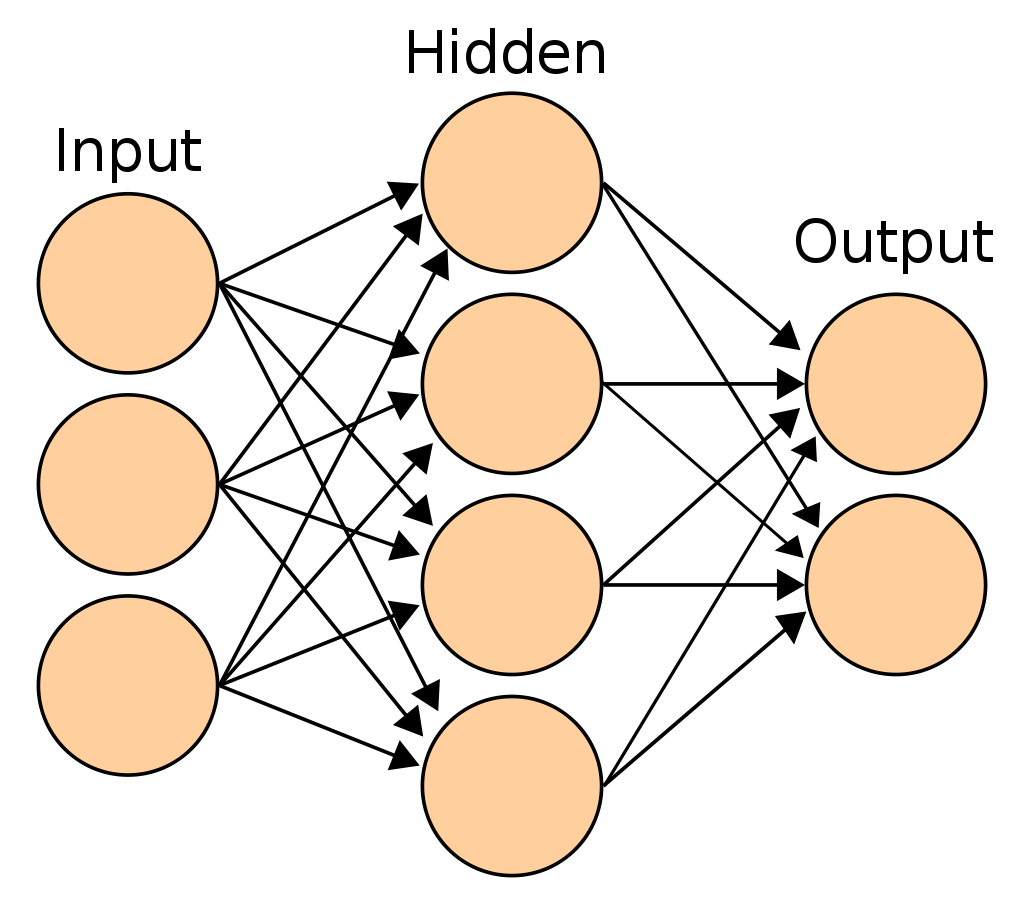
\includegraphics[scale=0.3]{ann_layers.png}}
	\caption{Przykładowa sieć neuronowa z trzema warstwami}
\end{figure}
\FloatBarrier

W przypadku sieci rekurencyjnej nie jest tworzona seria warstw komunikujących się ze sobą, a jedna rekurencyjna warstwa zmieniająca się w czasie. W celu lepszego zrozumienia struktury i sposobu działania takiej sieci często dokonywany jest proces rozwijania w czasie warstwy rekurencyjnej.

\begin{figure}[!ht]
	\centering
	\makebox[0pt]{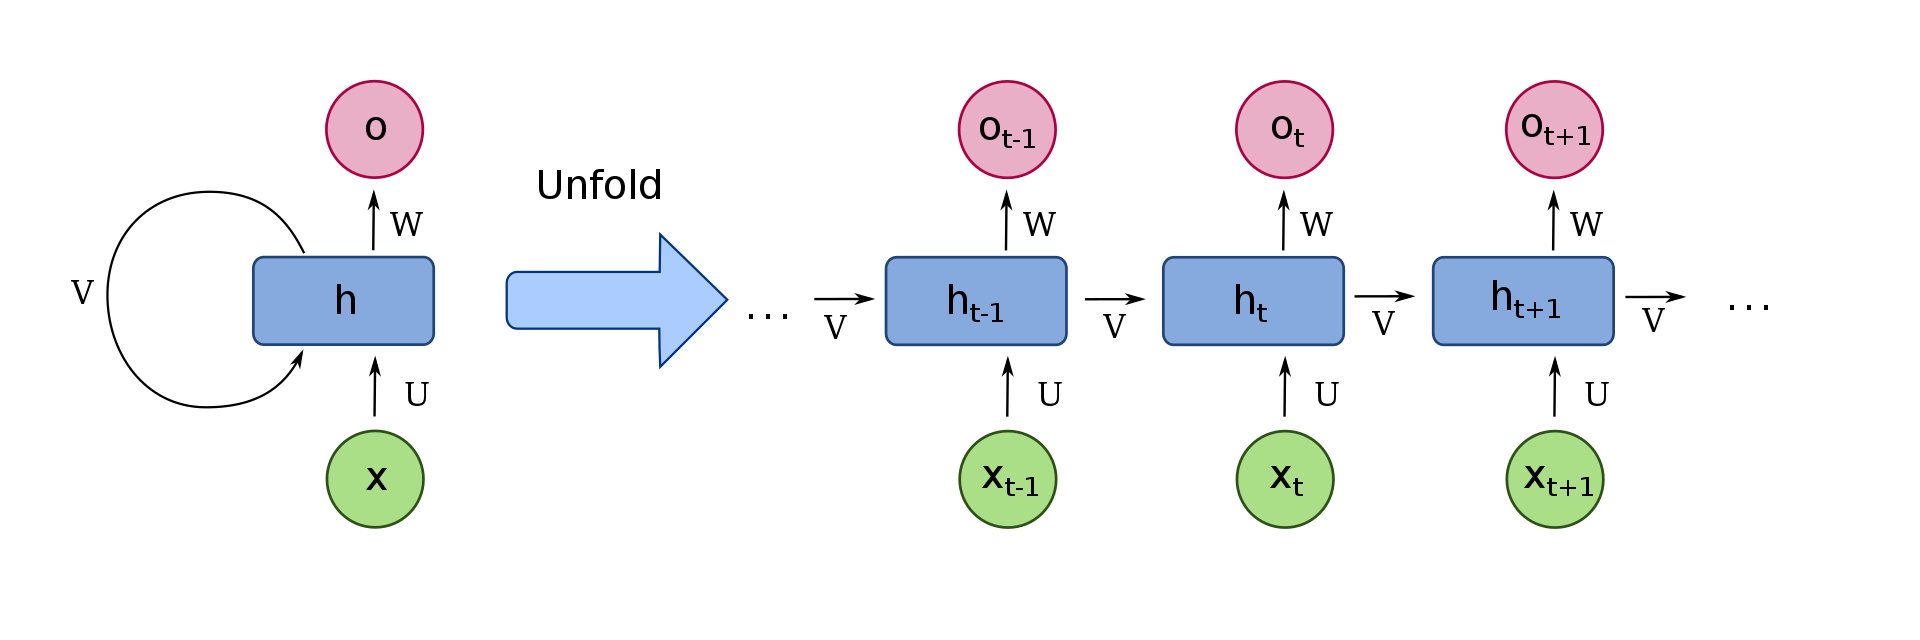
\includegraphics[scale=0.3]{Recurrent_neural_network_unfold.png}}
	\caption{Przykład rozwijania warstwy rekurencyjnej $h$}
\end{figure}
\FloatBarrier

W powyższym przykładzie należy zauważyć, że w wersji rozwiniętej $h_{t-1}, h_t i h_{t+1}$ nie są osobnymi warstwami, a jedynie reprezentacją warstwy $h$ w różnych krokach czasowych. 

Na przestrzeni lat powstało wiele wariacji na temat architektury rekurencyjnych sieci neuronowych odpowiadających na różne problemy i wymagania im stawiane. W dalszym ciągu pracy przedstawione zostaną wybrane architektury, które mogą zostać wykorzystane do rozwiązania postawionego problemu predykcji szeregu czasowego.


\subsection{Architektura LSTM}
Sieci Long Short-Term Memory(LSTM) powstały jako próba rozwiązania problemów występujących w klasycznych sieciach rekurencyjnych. Problemy te głównie dotyczyły aspektu rekurencyjnych sieci neuronowych pozwalającego ,,zapamiętać'' sieci poprzednie kroki czasowe. Zauważono, że korzystając z mechanizmu propagacji wstecznej przesyłany do następnych kroków czasowych sygnał błędu (sposób sieci na ,,zapamiętanie'' poprzednich przypadków) ma tendencję do znikania lub wybuchania. 

Zniknięciem sygnału błędu nazwać można sytuację, w której dąży on do zera w kolejnych krokach czasowych. Jest ona problemem w procesie uczenia, ponieważ może doprowadzić do bardzo dużego przedłużenia procesu lub nawet całkowicie uniemożliwić poprawne nauczenie sieci.

Wybuchem sygnału błędu nazywana jest sytuacja, w której dąży on do nieskończoności. Sytuacja ta jest niepożądana, ponieważ bardzo duży błąd przesyłany do następnych kroków czasowych oznacza, że sieć tak naprawdę niczego nie ,,zapamiętuje''. Może to prowadzić do oscylacji wag w sieci bez sygnału błędu stabilizującego wynik. 

Problemy te zostały podniesione przez S. Hochreiter'a w jego pracy doktorskiej, a następnie dokładniej opisane w roku 1991 we wspólnej pracy z J. Schmidhuber'em. 
W ramach artykułu ,,Long Short-Term Memory'' zaproponowali oni całkowicie nową architekturę rekurencyjnej sieci neuronowej dążącą do rozwiązania wyżej opisanych problemów \cite{hochreiter1997long}.

Stworzona została architektura oparta na komórkach pamięci i bramkach. Podstawową składową warstwy w tej architekturze jest komórka pamięci. Trzonem komórki jest rekurencyjna jednostka liniowa posiadająca Stałą Karuzelę Błędu (Constant Error Carousel), w skrócie CEC. Wartości CEC będą nazywane stanem komórki. Istnienie mechanizmu CEC eliminuje problemy z sygnałem błędu, ponieważ zapewnia on, że lokalny błąd nie będzie się samoistnie zmieniał w kolejnych krokach czasowych.

Mechanizmem odpowiedzialnym za modyfikację stanu komórki są bramki wejściowa i wyjściowa. Bramka wejściowa zajmuje się kontrolą przepływu nowych informacji do komórki. Oznacza to, że decyduje ona czy zachować obecny stan, czy nadpisać go nowymi informacjami. Można rozumieć zadanie bramki wejściowej jako określanie czy należy zapamiętać nową wiedzę lub uaktualnić istniejącą wiedzę. 

Bramka wyjściowa natomiast kontroluje przepływ stanu komórki na zewnątrz. Decyduje ona czy przechowywana przez komórkę wiedza jest warta przekazania innym komórkom do zapamiętania. Jej zadanie możemy rozumieć jako decyzję czy podzielić się swoją wiedzą z resztą komórek czy zachować ją dla siebie. 

\begin{figure}[!ht]
	\centering
	\makebox[0pt]{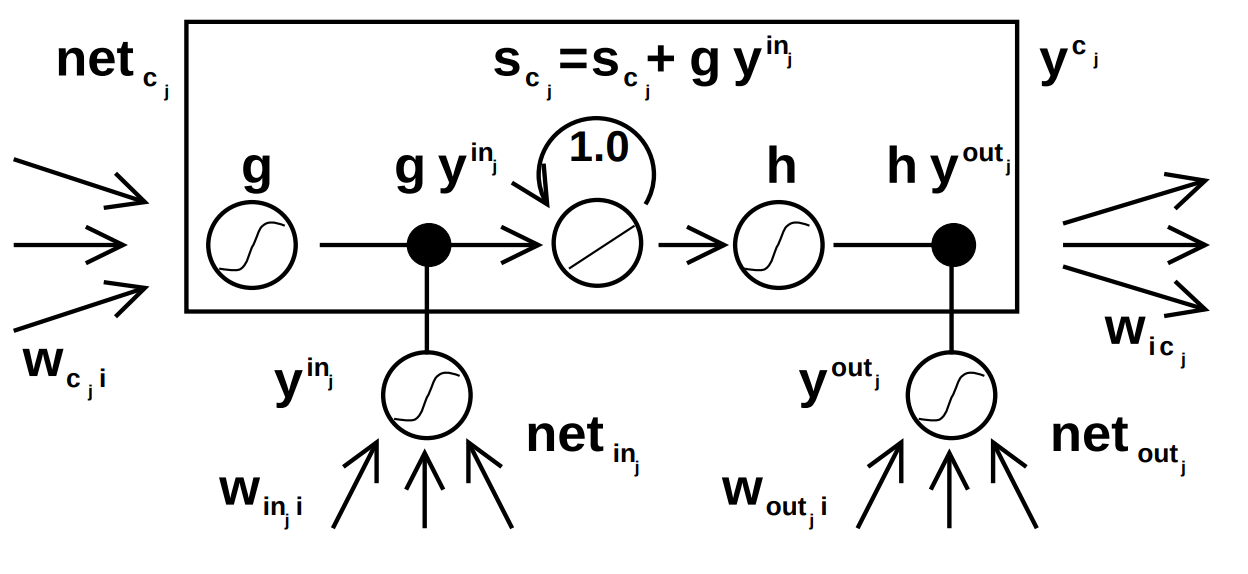
\includegraphics[scale=0.4]{lstm_without_forget_gate_schema.png}}
	\caption{Komórka pamięci w architekturze LSTM}
\end{figure}
\FloatBarrier

Na powyższym rysunku zauważyć możemy schemat budowy najprostszej komórki pamięci w sieci LSTM. Widzimy wyraźnie bramki wejściową i wyjściową operujące na sygnałach wejściowych $w_{in_ji}$, $y_{in_j}$, $net_{in_j}$ oraz wyjściowych ${w_{out_ji}}$, $y_{out_j}$, $net_{out_j}$. Widoczny jest również mechanizm zmiany stanu wewnętrznego komórki $s_{c_j}$ na podstawie przepuszczonego przez bramkę wejściową sygnału $y_{in_j}$.

Stworzona w taki sposób architektura okazała się mieć jeden poważny problem. Stan komórki wykazywał tendencje do liniowego wzrostu w kolejnych krokach czasowych. Wzrost ten mógł prowadzić do saturacji funkcji h. Saturacja ta prowadziła do przestania przyjmowania nowych błędów i zrównania wyniku komórki z wartością funkcji aktywacji bramki wyjściowej. W takich kierunkach komórka pamięci traciła swoje korzyści i wracała do zachowania typowego dla zwykłej sieci rekurencyjnej \cite{gers2000learning}.

Rozwiązaniem tego problemu okazało się dodanie trzeciej bramki nazywanej bramką zapominania. Zauważono, że przechowywanie w pamięci komórki danych przez bardzo długi często sprawia, że dane te są nieaktualne. Bramka zapominania kontroluje kiedy i ile przechowywanego stanu komórki $s_{c_j}$ należy zapomnieć. Dzięki usuwaniu z pamięci przestarzałych błędów wyeliminowany został problem saturacji funkcji h. Bramka zapominania stała się integralna częścią architektury LSTM. 

\begin{figure}[!ht]
	\centering
	\makebox[0pt]{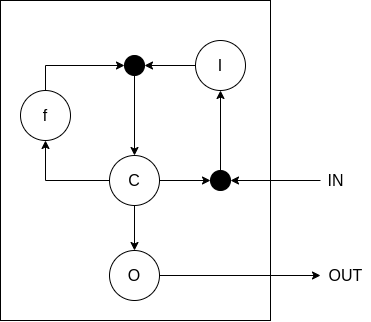
\includegraphics[scale=0.3]{lstm_with_forget_gate_schema.png}}
	\caption{Komórka pamięci w architekturze LSTM z bramką zapominania}
\end{figure}
\FloatBarrier

\subsection{Architektura GRU}
\subsection{Index of agreeement}

\section{Przygotowanie zbioru danych}
\subsection{Baza danych Instytutu Meteorologii i Gospodarki Wodnej}
\subsection{Baza danych Głównego Inspektoratu Ochrony Środowiska}
\subsection{Łączenie danych obu baz danych}
\subsection{Podział na geograficznie spójne szeregi czasowe}

\section{Przeprowadzone badania}
adsfjkhldsfh;dsaf
\subsection{Porównanie wydajności modeli predykcyjnych}
\subsubsection{Regresja liniowa}
\subsubsection{Drzewa decyzyjne}
\subsubsection{Prosta sieć rekurencyjna}
\subsubsection{Sieć rekurencyjna typu LSTM}
\subsubsection{Sieć rekurencyjna typu GRU}
\subsection{Badanie skalowalności modelu GRU}

\section{Otrzymane wyniki}
\subsection{Porównanie wydajności modeli predykcyjnych}
\subsubsection{Regresja liniowa}
\subsubsection{Drzewa decyzyjne}
\subsubsection{Prosta sieć rekurencyjna}
\subsubsection{Sieć rekurencyjna typu LSTM}
\subsubsection{Sieć rekurencyjna typu GRU}
\subsection{Badanie skalowalności modelu GRU}adsfds

\section{Wnioski}
sera
\printbibliography

\end{document}